\chapter{Interaktiv planlægning}
\label{chap:is}
Interaktiv planlægning (\is) er det sidste anvendelsesområde, vi vil belyse med henblik på at indføre tid i \pycsp. Det har dog vist sig, at emnet kun er sparsomt berørt i litteraturen, og der er ikke en klar definition på, hvad det er, og hvor det anvendes. 
%og at de få definitioner af \is vi har fundet, ikke er et selvstændigt anvendelsområde, men en definition af RTP med en hard deadline uden at være et kritisk system. \cite{?}. 
Vi forventede, at dette anvendelsesområde var brugt i forbindelse med computerspil, men efter at have studeret litteraturen og have rådført os med Lektor Kenny Erleben, der underviser på Det Danske Akademi for Digital Interaktiv Underholdning (DADIU), er vi kommet frem til, at der ikke findes en udbredt definition af \is. Han fortæller desuden, at en af begrundelserne for, at computerspilfirmaerne ikke er interesserede i at oplyse om deres metoder til at planlægge begivenheder i spil, er at det  betragtes som en  forretningshemmelighed. 

Vi vil derfor i stedet på baggrund af en række praktiske eksempler indkredse, hvad vi forventer, \is skal kunne bruges til, og på baggrund af eksemplerne se på muligheden for at implementere en model i \pycsp. Dette kapitel adskiller sig dermed væsentligt fra de foregående to kapitler, i og med anvendelsesområdet ikke baserer sig på en fast definition givet af litteraturen, og vi ikke bygger på kendt viden.

\section{Eksempler}
Vi har valgt to scenarier, som vi forventer med fordel kan benytte \is. Det første er en repræsentation af et ur, hvilket vi mener, er det simpleste eksempel, der kan gøre brug af \is. Det andet eksempel er en del af et computerspil, som er vores forventede primære anvendelsesområde for \is. 

\subsection{Et ur}
Det første eksempel på \is er en repræsentation af et digitalur. Uret består af seks cifre, og en gang i sekundet skal sekunderne tælles op. Det er et krav, at en opdatering skal sætte uret til at vise det korrekte tidspunkt. Vi forestiller os, at uret er en del af et større system, hvor der er andre ressourcekrævende begivenheder, der er vigtigere at få udført end opdateringen af uret. Opdatering af uret foregår ved at planlægge en begivenhed til hvert sekund, der specificerer, hvad uret skal vise. Da det har en lav prioritet, er der ikke nogen garanti for, at denne begivenhed indtræffer i det sekund, den er planlagt til. Derfor skal begivenheden  bortkastes, såfremt den overskrider sin deadline. Deadlinen er et nyt sekunds begyndelse, for at sikre den krævede korrekthed. 

Uret er repræsentativt for \is, da der planlægges en række begivenheder, der skal foregå i fremtiden og hver især har tilknyttet en deadline.

\subsection{Computerspil}
Et andet eksempel, \fxnote*{hvorfor?}{vi mener repræsenterer  \is}, er mere realistisk og bunder i vores oprindelige forventning om, at \is  var defineret af computerspilindustrien, som en metode til at planlægge, hvordan spil kan forløbe. Uden deres definition af \is vil vi i stedet opstille et hypotetisk eksempel. 

Vi forstiller os et computerspil, der er skrevet i \pycsp, og hvor hvert element i spillet er en selvstændig proces. I dette computerspil skal der være en fugl, der jævnligt flyver på tværs af skærmen. Fuglen skal starte på et given tidspunkt og med en fast hastighed bevæge sig over skærmen. Fuglens \fxnote*{ordvalg}{flugt} over skærmen udregnes af to typer processer, baseret på en model, der minder om videokomprimering. Den første procestype er en højprioritetsproces, der står for at udregne positionen af fuglen med  et fast interval. Den anden procestype kan bestå af mange lavprioritetsprocesser. Hver lavprioritetsproces står for en egenskab ved fuglen, som  f.eks. optimere animationen af fuglen, tilknytte fuglekvidren og andre ikke essentielle egenskaber. Den højtprioriterede proces udføres sjældent, men er essentiel at få udført, mens lavprioritetsprocesserne blot skal udføres, hvis der er mulighed for det og ellers skal droppes.

\section{Beskrivelse}
Vi kan se på hvilke egenskaber eksemplerne har, og hvilke krav de derved stiller for at kunne håndteres i et programmeringssprog. Først og fremmest ligger eksemplerne  inden for realtidsmodellen. Ligeledes skal der være mulighed for at tilknytte en deadline til en begivenhed. Dette vil i vores opstillede eksempler være hard deadlines, men vi kan ikke udelukke at der findes eksempler hvor andre typer deadlines vil være fordelagtige. Eksemplet med computerspillet viser at der er behov for at tilknytte en prioritet, der er uafhængig af deadline, til en begivenhed. Dette har vi diskuteret som en mulig udvidelse til RTP i \cref{sec:deadlineFuture}. Disse egenskaber minder alle om dem der er er givet for RTP. Ud over disse skal vi også kunne planlægge en begivenhed. Det lægger sig mere op af \des med det forbehold at vi i \is ikke garanterer at en begivenhed sker på et bestemt tidspunkt, men tidligst på det angivne tidspunkt.  

Vi kan dermed se \is som en blanding af RTP og \des, med tidsmodellen og deadlines fra RTP, og planlægningen af begivenheder fra \des. 

%\is arbejder ligesom RTP i realtid. Desuden minder de også om hinanden da man i begge modeller arbejder med begivenheder, der har tilknyttet deadlines. For det tredje viser computerspilseksemplet at en udvikleren skal kunne tilknyttes prioriteter til begivenheder, der skal sættes uafhængigt af deres deadline i \is. Dette nævnte vi som en mulig udvidelse til RTP i \cref{sec:deadlineFuture}.

%\is og \des minder også om hinanden da man i begge modeller skal kunne planlægge en begivenhed til at foregå ud i fremtiden. Men hvor \des kan garantere at begivenheden sker på præcist det angivne tidspunkt kan vi i \is kun garantere at det sker efter et givent tidspunkt.

\section{Design og implementering} 

Da kravene til \is rent praktisk ligger meget tæt op af de løsninger, vi tidligere har beskrevet, i RTP, vil vi ikke implementere en selvstændig \ip-version. Vi vil i stedet udvide RTP-versionen med den krævede funktionalitet så RTP kan foretage både RTP og IP.
Vi skal derfor udvide RTP så man kan planlægge begivenheder der skal foregå ud i fremtiden, samt sætte en prioritet på en proces uafhængigt af processens deadline. 

%I \des kom vi frem til at planlægningen af begivenheder ud i fremtiden også kan tolkes som en venten. Dermed kan man se på \is som en udvidelse til RTP, hvor man udover at have mulighed for at sætte en deadline skal have mulighed for at vente. For at kunne bruge RTP til \is vil det desuden være hensigtsmæssigt at  udvide RTP så det er muligt for udvikleren at tilknytte en prioritet til begivenheden.

\subsection{Funktionerne \code{Now} og \code{Wait}}

Vi argumenterer i kapitel \ref{chap:des} for, at planlægning af begivenheder til et givet tidspunkt kan tolkes som venten indtil tidspunktet. Vi vil derfor også i forbindelse med \ip introducere de to globale funktioner \code{Now} og \code{Wait}, der hhv. returnerer den aktuelle tid og lader en proces vente i et givent tidsrum. Vi har til \is ændret den interne implementering af funktionerne, så de bruger realtid. Ved at bruge de samme funktioner, sikres en ensartet implementering af tid på tværs af TimedPyCSP, og man kan i vores øjne med fordel tilføje funktionen \code{Now} til alle \pycsp versionerne for på den måde at ensrette de forskellige implementeringer. Hvis \code{Now} blev inkluderet i \code{greenlets}-versionen, kunne den fjernes helt fra denne version, da de baserer sig på den samme tidsmodel, nemlig realtid.

Forskellen i implementering mellem versionen, der benytter realtid som tidsmodel, ifht. til versionen der bruger diskrettid som tidsmodel, er simpel. I stedet for at \sched en kender tiden, og at det derfor er dennes tid, vi returnerer i diskret tid, bruger vi nu Pythons \code{time}-modul. Genimplementeringen består derfor  i at ændre funktionen \code{Now} til at bede \code{time}-modulet om det nuværende tidspunkt. Implementeringen af \code{Wait} benytter sig af \code{Now} til de tidsspecifike operationer, hvorfor vi kan genbruge denne funktion, uden en eneste ændring. 

\subsection{Udvikler"-prioriteter}
I computerspilseksemplet, har processerne forskellige prioritet dikteret af udvikleren. Denne prioritet er ikke det samme som den prioritet, der allerede findes i RTP, da denne  er beregnet af \sched en. For at adskille dem vil vi kalde udviklerens prioriteter for udvikler-prioritet. Vi skal udvide RTP således at det kan håndtere processer, der både kan have deadlines og udvikler"-prioriteter tilknyttet. Dette har vi allerede beskæftiget os med i \cref{sec:deadlineFuture}, som en fremtidig mulighed for RTP. 

Først skal det fastlægges i hvilket interval udvikler-prioriteter kan antage. Vi ønsker ikke at begrænse udvikleren ved at have for få prioriteter, men omvendt reduceres \sched ens  mulighed for at udvælge processer hvis hver proces har sin egen unikke prioritet. Hvis en udvikler kan vælge mellem et stort antal prioriteter risikere man også at introducere en prioritetsskrue. Dette sker hvis en udvikler flere gange undervejs i udviklingen af et program øger den maksimale prioritet, da han mener den nuværende proces er den vigtigste uden at gennemtænke det i relation til alle andre processer. Dermed risikerer man at udvande prioriteten for de allerede udviklede processer.  Der skal derfor være en maksimal prioritet, og intervallet man kan angive prioriteter i, må ikke være så stort at processerne for unikke prioriteter.\fxwarning{omskriv det med unikke prioriteter}

Præcis  hvor stort intervallet skal være for udvikler"-prioriteter, kræver dog en bredere analyse af flere projekter, og vi vil derfor begrænse os til at lave et foreløbigt interval på ti, man senere nemt vil kunne ændre baseret på en bedre analyse.


I RTP-versionen er \sched en en EDF algoritme, som kun planlægger processerne på basis af deres deadline. Vi kan derfor ikke bruge den samme skemaplanlægningsalgoritme, men skal udvide \sched en. For at udvide \sched en skal vi definere den indbyrdes relation mellem deadlines og udvikler"-prioriteter. Baseret på computerspil-eksemplet kan vi se,  at de processer, der har  tilknyttet en udvikler"-prioritet, skal gå forud for både de processer, der har tilknyttet en deadline, og dem der hverken har prioritet eller deadline. 

I RTP  indeholder \sched en alle processer med en prioritet i en enkelt hob kaldet \code{has\_priority}. Vi kan udvide denne hob til en sorteret liste af hobe, en for hver prioritet. Med en liste af hobe vil hver hob være lille, og dermed vil de enkelte operationer på hoben være hurtigere. \Sched en kan desuden bruge EDF på hver hob da alle processerne i hver hob har samme prioritet. For at udvælge hvilken proces der skal aktiveres vælges det første element i den første ikke-tomme hob. 
%Til at udvælge hvilken hob der skal udvælges en proces fra løbes listen igennem efter den hob med de højst prioriterede processer, der har elementer. 
Alternativt kan vi udvide den ene hob, der allerede findes, så alle processer både med og uden udvikler"-prioritet befinder sig i den samme hob. Med denne metode kan man ikke bruge EDF, men der skal udvikles en funktion, der kombinerer  udvikler"-prioriteten og deadlinen til en endelig prioritet. Man vil så kunne bruge en Least Priority First (LPF) algoritme, der fuldstændigt svarer til EDF, men baserer udvælgelsen på prioritet. I sagens natur vil denne hob  være større end, hvis man brugte en liste af hobe. Dette er dog ikke et stort problem, da hoben gemmer data i en træstruktur, og søgetiden vokser derfor logaritmisk til antallet af elementer. Vi antager derfor, at forskellen mellem de to fremgangsmåder ikke vil være nævneværdig, og under alle omstændigheder vil den ikke være anderledes end i \code{RTP}-versionen, hvor der også kun findes en hob. Fordelen ved kun at bruge en hob er, at vi kan genbruge \code{has\_priority} hoben og  ikke skal lave en større omskrivning af \code{RTP}-versionen. Desuden skal vi ikke lineært gennemløbe en liste af hobe for at finde den første hob med elementer, men kan med det samme starte i den korrekte hob. Endnu en fordel ved denne metode er, at vi nemt kan  ændre vores oprindelige antagelse om, at prioritet skal gå forud for deadlines, blot ved at ændre på den eksterne funktion, der kombinerer de to parametre.

Vi mener, at fordelene ved kun at have en hob og muligheden for at kunne ændre på vægtningen af forholdet mellem udvikler-prioritet og deadline, er større end besparelsen i tid ved at have flere hobe, der skal vedligeholdes. Derfor vælger vi  at genbruge \code{has\_priority}, som den eneste hob til  processer, der har deadlines og udvikler"-prioritet. Med kun en hob skal vi derfor udvikle en ekstern funktion, der kombinerer to tal til en endelig prioritet. Denne funktion skal sikre at at prioriteten sat af udvikleren altid vil være dominerende. Det bør nævnes at jo højere udvikler-prioriteten er, jo vigtigere er processen. I implementeringen af \code{has\_priority} bruges der en min-hob, hvorfor vi internt inverterer udvikler"-prioriteten, så 0 er den højeste prioritet, og processer, hvor udvikleren ikke har angivet en prioritet, sættes til 10.

Vi har valgt at implementere en simpel løsning, hvor  de to tal lægges efter hinanden. Hvis man eksempelvis har en udvikler"-prioritet på 2 og en deadline på 20, sættes de efter hinanden, så den endelige prioritet bliver 220. Dette kan vi gøre, da antallet af cifre i hhv. deadlines og udvikler-prioritet ligger fast, så vi risikerer ikke en forskydning, når de lægges efter hinanden. For at sikre at processer, der har en udvikler"-prioritet, og ingen deadline, også kan planlægges, bruges der en kunstig høj deadline. Ønsker man en anden løsning for at sammenholde prioriteter og deadlines, kan det nemt opnås blot ved at ændre i en enkelt funktion.
    
\section{Evaluering}
Vi har i det foregående afsnit beskrevet hvad der skal til, for at implementere \is i \pycsp. Vi vil i dette afsnit gennemgå hvordan \is kan implementeres, for derefter at evaluere vores løsning med udgangspunkt i ureksemplet.
\fxnote{Korrekthed}
Netværket er struktureret som vist på \cref{fig:watch_network}. Som vi kom ind på tidligere, har vi en ur-proces, en række tidsstempel-processer, og nogle dummy-processer. Ur-processen modtager et tidstempel fra alle  tidsstempel-processerne, og står for at at opdatere uret ud fra disse. Tidsstempel-processerne modtager fra start, hvert sit tidsstempel, som de planlægger at sende i fremtiden når tidspunktet er korrekt. Hver tidsstempelproces  venter indtil dette tidspunkt, for så at sende tidspunktet til ur-processen. Samtidigt med at uret skal holdes opdateret, køres der også en række dummyprocesser i par, som kommunikerer med hinanden. Hver dummyproces udregner 50.000 iterationer i en simpel estimering af $\pi$, og på testmaskinen tager dette i gennemsnit 0.07707 sekunder med en standardafvigelse på 0.01245 sekunder. Dummyprocesserne brugte vi også i slagterieksemplet.
\begin{figure}
 \begin{center}
  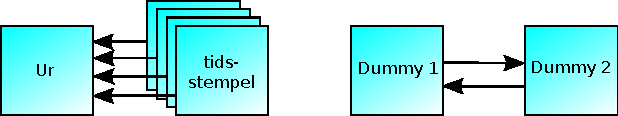
\includegraphics[scale=1]{images/watch-network}
	\caption{Procesnetværk med flere konverteringsprocesser, og analyseprocesser. Dummyprocessernes kørsel foregår uafhængigt af uret, og tidsstempelprocesserne, men alle processerne køres samtidigt.}
	\label{fig:watch_network}
\end{center}
\end{figure}

I \code{greenlets}-versionen har vi ikke mulighed for direkte at planlægge en begivenhed i fremtiden. Vi kan dog oprette en separat tråd  via \code{IO}-dekoratøren. I den separate tråd kan man så vente via funktionen \code{sleep}. Dette er den eneste metoden for processer at afgive kontrollen i et tidsrum i \emph{greenlets}-versionen uden at blokere for hele programmet, og metoden er beskrevet på  hjemmesiden for \pycsp. Metoden medfører dog et overhead, da der skal oprettes en ny tråd blot for at vente.  Med introduktionen af \code{Wait}, bliver processen lagt på \code{timers}-hoben, og det er derfor ikke længere krævet at oprette en separat tråd til en proces der ønsker at vente. En udvikler der skal planlægge en proces til senere kørsel, slippe derfor i RTP for at skulle introducere koden vist i \cref{fig:sleep} før en proces kan planlægges.

\begin{lstlisting}[firstnumber=1 ,float=hbtp, label=fig:sleep, caption=Funktion der venter et antal sekunder]
@io
def sleep(n):
    import time
    if n>0: time.sleep(n)
\end{lstlisting}
 
Ved implementeringen af \code{greenlets}-versionen, opstår der et problem i opdateringen af uret. Begrænsningen om kun at opdatere uret så længe tidsstemplet er korrekt, viser sig nemlig problematisk at implementere. I den første version fulgte vi eksemplet og implementeret kontrollen i tidsstempel-processen, med en \code{alternation}, og en \code{timeout}-guard.  Tidsstempel-processen, skal derfor inden et sekund have sendt beskeden til uret, og vil ellers helt droppe forsendelsen. Resultatet af denne implementering kan man se af linje 1 i \cref{tab:watch}. Den gennemsnitlige forsinkelse på 1.529 sekunder burde være umulig, da opdateringer på over et sekund bør falde bort. Grunden til, at forsinkelsen ikke falder bort, er at tidsstempel-processen korrekt får overført tidsstemplet til urprocessen inden for et sekund. Ur-processen bliver efterfølgende lagt på \code{next} listen da den er klar til at blive kørt, og har modtaget tidsstemplet. Nu skal den så slås, for at blive udvalgt af \sched en, på lige fod med de dummy-processer, der også er klar til at blive kørt. Når ur-processen bliver udvalgt er tiden forpasset og uret bliver opdateret for sent.
Vi har derfor lavet endnu en version, hvor ur-processen også kontrollere, at tiden ikke er forpasset. Resultatet af denne ændring ses af linje 2 i tabellen, hvor vi kan se, at uret ikke når at blive opdateret en eneste gang, inden tiden er forpasset.
\begin{table}[htbp]
	\centering
	\begin{tabular}{l>{\centering\arraybackslash}p{3.1cm}>{\centering\arraybackslash}p{3.1cm}>{\centering\arraybackslash}p{3.1cm}}
       	\toprule
        \mc{Version}     & Rettidige tidsopdateringer(\%)&Gennemsnitlig forsinkelse(s)&Standard Afvigelse \\
        \midrule
        Greenlets ver. 1 & 0  & 1.529 & 0.276 \\ 
        Greenlets ver. 2 & 0  & NaN   & 0\\
        RTP (100 opdateringer) & 80 & 0.539 & 0.411 \\
        RTP (50 opdateringer) &100 & 0.077& 0.023\\
        \bottomrule
    \end{tabular}
	\caption[]{Proces-netværk betstående af et ur, 100 opdateringer, og baggrundsprocesser }\\
	\label{tab:watch}
\end{table}

De to forskellige implementeringer af \code{greenlets}-versionen viser tydeligt hvorfor den ikke er egnet til planlægge processer, der skal aktiveres inden for en tidsperiode. Problemet er, at selvom tidsstempel-processerne sender sit data til ur-processen inden for tidsgrænsen, skal ur-processen stadig vente på at blive aktiveret, på lige fod med alle dummy-processerne. I greenlets-versionen aktiverer  \sched en processerne ud fra en FIFO strategi, og ur-processen vil derfor komme sidst i køen af processer, der ønsker at blive aktiveret. 

I modsætning til \code{greenlets}-versionen, og dens FIFO strategi ser vi i tabellen for \code{RTP}-versionen at den  når 80\% af tidsstemplerne. Værd at bemærke er at den gennemsnitlige forsinkelse i \code{RTP}-versionen kun indeholder forsinkelsen for de tidsstempler der ankom rettidigt, hvorfor tallet er svært at sammenligne med \code{greenlets}-versionen. Det mest bemærkelsesværdige ved \code{RTP}-versionen er at forsinkelsen og standardafvigelsen er meget høj. Dette passer ikke sammen med vores forventning om at ur-processen kommer til som den første proces, og derfor kun bør være forsinket med tiden det tager for kørslen af en  dummy-proces.

Efter at have analyseret kørslen er vi kommet frem til at problemet skyldes prioritetsnedarvning, nærmere bestemt at vi ikke korrekt får nedprioriteret ur-processen igen, efter den har modtaget en opprioritering fra en tidsstempel-proces. Den gamle prioritet bliver efterfølgende fejlagtigt overført til tidsstempel-processer der aktiveres på et senere tidspunkt. Som antallet af tidsstempel processer aktiveres, vil tidsstempel-processer modtage flere og flere nedarvede-prioriteter, hvorved mere og mere tid bruges på prioritetsnedarvning. Vi kan konstatere at det er det samme problem som vi kom ind på i \cref{sec:rtp_evalation}, og vi forventer at en korrektion af prioritetsnedarvning vil løse problemet. 

Da problemet vokser med antallet af tidsstempel-processer der startes har vi en forventning om at hvis der startes færre tidsstempel-processer vil fejlen ikke gøre en målbar forskel. Vi foretog derfor en test med kun 50 tidstempel-processer for at minimere problemet, og resultatet ses af linje 4 i \cref{tab:watch}. Her kan vi se at  den gennemsnitlige forsinkelse tidstemplerne ankommer med, svarer til kørslen af en dummy-proces, hvilket er forventet, da vi ikke har preemptiv kontekstskift, og derfor nødvendigvis må afslutte en dummy-proces før tidsstempel-processen bliver aktiveret. 

På baggrund af testen forventer vi at når fejlen er løst, vil \code{RTP}-versionen kunne skalere frit og stadig have en gennemsnitlig forsinkelse og SA der er sammenlignelig med eksemplet hvor der kun er 50 opdateringer.
\fxnote{Eval af prioritet}
\section{Opsummering}

Vi har i dette kapitel gennemgået to eksempler for at indkredse en definition af interaktiv tid og er kommet frem til at det ikke er et selvstændigt anvendelsesområde, men ligger tæt op af RTP, hvorfor vi har udvidet RTP til at kunne foretage interaktiv planlægning.

Ud fra eksemplerne har vi identificeret at der mangler at blive implementeret  planlægning af begivenheder, og prioritet af processer i \code{RTP}-versionen. Vi har implementeret den manglende funktionalitet, og for udviklerne introduceret funktionerne \code{Wait},  \code{Now} og \code{Set\_priority}. Ved at introducere funktionaliteten direkte i RTP, opnår vi desuden at også RTP-versionen kan drage nytte af denne funktionalitet, som det ses af \cref{tab:dummy-run}, hvor dummy-processer blev introduceret til slagterieksemplet.

Implementeringen af eksemplet har vist, at man nemt kan planlægge processer til at have begivenheder, der skal foregå i fremtiden, samt foretage en skemaplanlægning, der sørger for  rettidigt, at få eksekveret de processer, der har en deadline. Implementeringen af eksemplet har også afdækket en fejl i vores implementering af prioritetsnedarvning, der medfører, at når antallet af processer stiger, falder effektiviteten. Vi har i den forbindelse fundet frem til, at det er den samme fejl, som vi har identificeret i RTP og forventer at løsning af denne fejl, vil medføre at der kan planlægges et vilkårligt antal processer.
